\documentclass{article}
\usepackage{amsmath}
\usepackage{tikz}
\usepackage{graphicx} % Required for inserting images

\newtheorem{definition}{Definition}[section]

\title{Probability Theory Notes}
\author{Alex Gregory}
\date{July 2023}

\begin{document}

\maketitle

\section{Bernoulli}

Suppose we flip a coin ten times. What is the probability we get three heads? My first guess would be 0.3. In this section, we will see that this is not the case. In order to calculate this probability, we first need to discuss permutations and combinations.

\subsection{Permutations}

Suppose we toss five coins and count the number of heads we get. Let $X$ be a random variable with the following outcomes $X = \{h_1, h_2, h_3, h_4, h_5\}$  where $h_i$ represents getting a heads on the $i$-th toss.

\section{Permutations}

Suppose we have a set of five characters $X = \{ A, B, C, D \}$. Suppose we select two characters at random from $X$ without replacement, how many possible combinations of characters are there?

For the first character, $c_1$, there are 4 possible outcomes: $A$, $B$, $C$, or $D$. For the second character, $c_2$, there are 3 possible outcomes depending on the $c_1$. Let us visualise these outcomes as a tree.

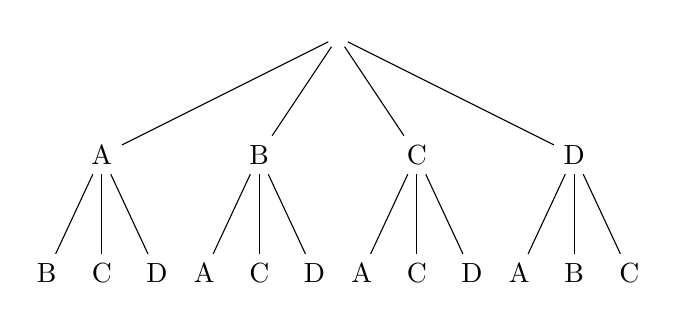
\begin{tikzpicture}
[
    level 1/.style = {sibling distance = 2cm},
    level 2/.style = {sibling distance = 0.7cm},
]
\node {} [sibling distance = 2.5cm]
    child {
        node {A}
        child {node {B}}
        child {node {C}}
        child {node {D}}
        edge from parent
    } 
    child {
        node {B}
        child {node {A}}
        child {node {C}}
        child {node {D}}
        edge from parent
    } 
    child {
        node {C}
        child {node {A}}
        child {node {C}}
        child {node {D}}
        edge from parent
    } 
    child {
        node {D}
        child {node {A}}
        child {node {B}}
        child {node {C}}
        edge from parent
    };
\end{tikzpicture}

From the tree above, it is clear there are $4 \cdot 3 = 12$ permutations. In general, if you have a game where there are $m$ steps and at each step, $i$, there are $n_i$ choices the total number of permutations is,
$$
    n_1 \times n_2 \times \dots \times n_m.
$$

\section{Combinations}

A combination is like a permutation but where the order is not important. So, where before we counted $AB$ as different to $BA$, now we treat them as the same.

Suppose again we have the set $X = \{ A, B, C, D \}$ and we select two characters at random without replacement. We know from the previous section there are $4 \cdot 3 = 12$ permutations of $X$. The possible permutations are as follows,
$$
\begin{matrix}
    AB & BA \\
    AC & CA \\
    AD & DA \\
    BC & CB \\
    BD & DB \\
    CD & DC \\
\end{matrix}
$$
Notice in the list of permutations each combination is repeated twice, for example $AB$ and $BA$. Therefore, if we divide the total number of permutations by the number of times each combination is repeated, we get the total number of combinations. For the example, this number of combinations is,
$$
\frac{4 \cdot 3}{2} = 6
$$
How do we find the number of times each combination is repeated in the list of permutations? Suppose for $X$ we want to know the number of times the combination $AB$ is repeated. $A$ can appear in the first or second position. Depending on the position of $A$, there is only one place where $B$ can be. So, the combination $AB$ is repeated, $2 \cdot 1 = 2$ times. The characters $AB$ are not important, in-fact any combination of characters is repeated $2$ times.

Suppose now that we select three characters from $X$ without replacement rather than two. The number of permutations is $4 \cdot 3 \cdot 2 = 24$. Consider the combination $ABC$. Again, again can be in the first, second or third position. Depending on the position of $A$, $B$ can be in two positions. Finally, depending on the position $A$ and $B$, $C$ must be in the remaining position. So each combination is repeated $3 \cdot 2 \cdot 1 = 6$ times. So, overall there are,
$$
    \frac{4 \cdot 3 \cdot 2}{3 \cdot 2 \cdot 1} = \frac{24}{6} = 4,
$$
combinations. The list of combinations are as follows,
$$
\begin{matrix}
    ABC \\    
    ABD \\
    BCD \\
    CAD \\
\end{matrix}
$$
Now consider the more general case. Suppose our set, $X$ has $n$ elements, and we want to find the number of combinations of length $r$ we can get from $X$. In English, the number of combinations is,
$$
\text{Number of combinations} = \frac{\text{Number of permutations}}{\text{Number of times each combination is repeated}}
$$
The number of permutations is $\frac{n!}{(n - r)!}$. The number of times each combination is repeated is $r!$. So, our formula becomes,
$$
\text{Number of combinations} = \frac{n!}{(n - r)!r!} = 
\begin{pmatrix} n \\ r \end{pmatrix}.
$$
The symbol $\begin{pmatrix}n \\ r\end{pmatrix}$ is referred to in English as $n$ choose $r$.

\subsection{Binomial Distribution}
Suppose we flip a coin 10 times. What is the probability we get $3$ heads? Naive guess might be 0.3 but we will see that is not the case.

We could get three heads in the first three tosses.
$$
    HHHTTTTTTT
$$
The probability of this event is $0.5 ^ {10}$. Equally, we could get the heads in the final three tosses.
$$
    TTTTTTTHHH
$$
The probability of this event is again $0.5 ^ {10}$. Since we are throwing a fair coin, the probability of any combination of ten heads and tails is $0.5 ^ {10}$. So, the probability of getting three heads is $0.5 ^ {10}$ multiplied by the number.

To count the number of combinations of three heads in ten tosses, we can use $n$ choose $r$ where $n$ is 10 and $r$ is three. The number of combinations is,
$$
    \begin{pmatrix}10 \\ 3\end{pmatrix} = \frac{10!}{7!3!} = \frac{720}{6} = 120
$$
Therefore, the probability of getting a three heads in ten tosses is,
$$
    120 \cdot 0.5 ^ {10} = 0.1171875
$$
Why do we count the number of combinations and not the number of permutations? First, label the heads of each coin toss as $X = \{ H_1, H_2, \dots, H_{10} \}$. The number of length three permutations for $X$ is,
$$
    10 \cdot 9 \cdot 8 = 720.
$$
However, this counts $\{ H_1, H_2, H_3 \}$ and $\{ H_2, H_1, H_3 \}$ as two separate outcomes. Counting these as two separate outcomes is not important to us as both mean the same thing i.e the first three tosses were heads.

In general, the formula for getting $i$ successes from $n$ trials is,
$$
    P(X = i) = \begin{pmatrix} n \\ i \end{pmatrix} p ^ {i} p ^ {n - i}.
$$
We also have a set of conditions such that a binomial distribution can be used:
\begin{itemize}
    \item The number of observations $n$ is fixed.
    \item The probability $p$ does not change during the experiment.
    \item The outcomes of each observation is either success or failure (heads or tails).
    \item Each observation is independent on one another.
\end{itemize}

\section{Poisson Distribution}

Suppose we have a very bias coin which has a very low probability of being heads. Suppose we flip this coin an infinite number of times. How long do we have to wait until we get $k$ heads?

Creating a tree diagram for three coin tosses is a lot of work let alone an infinite number of coin tosses so we cannot do this with a diagram. The binomial distribution works only for a fixed number of coin tosses so we cannot use that without some work. Let us work out what happens when the number of coin tosses, $n$, tends to infinity. Let us start by defining the following quantity, 
\begin{equation*}
    \lambda = p * n.
\end{equation*}
Where $p$ is the probability of getting heads and $k$ is the number of coin tosses. Let us plug this into the formula for the binomial distribution and give a limit as $n$ approaches infinity.
\begin{align*}
    P(X = k) & = \lim_{n \rightarrow \infty} \frac{n!}{k!(n - k)!}p^k(1 - p)^{n - k} \\
             & = \lim_{n \rightarrow \infty} \frac{n!}{k!(n - k)!} \left(\frac{\lambda}{n}\right)^k \left(1 - \frac{\lambda}{n} \right)^{n - k} \\
             & = \frac{\lambda ^ k}{k!} \lim_{n \rightarrow \infty} \frac{n!}{(n - k)!} \frac{1}{n^k} \left(1 - \frac{\lambda}{n} \right)^{n - k} \\
             & = \frac{\lambda ^ k}{k!} \lim_{n \rightarrow \infty} \frac{n!}{(n - k)!} \frac{1}{n^k} \left(1 - \frac{\lambda}{n} \right)^{n - k} \\
             & = \frac{\lambda ^ k}{k!} \lim_{n \rightarrow \infty} \frac{n!}{n^k(n - k)!} \left(1 - \frac{\lambda}{n}\right)^{-k}\left(1 - \frac{\lambda}{n} \right)^{n} \\
\end{align*}
Now we calculate the limits of each term separately. For the first term, we have,
\begin{equation*}
    \lim_{n \rightarrow \infty} \frac{n!}{n^k(n - k)!} = \lim_{n \rightarrow \infty} \frac{n(n-1)(n-2)\dots(n-k+1)}{n^k} = 1
\end{equation*}
For the second term, we have,
\begin{equation*}
    \lim_{n \rightarrow \infty} \left(1 - \frac{\lambda}{n}\right)^{-k} = (1 - 0) ^{-k} = 1
\end{equation*}
For the final term, we use the fact that,
\begin{equation}
    \lim_{n \rightarrow \infty} \left( 1 + \frac{x}{n} \right)^n = e^x
\end{equation}
By letting $x = - \lambda$, we get,
\begin{equation}
    \lim_{n \rightarrow \infty} \left( 1 - \frac{\lambda}{n} \right)^n = e^{-\lambda}.
\end{equation}
Finally bringing it all together,
\begin{align*}
P(X = k) = \frac{\lambda ^ k}{k!} \lim_{n \rightarrow \infty} \frac{n!}{n^k(n - k)!} \left(1 - \frac{\lambda}{n}\right)^{-k}\left(1 - \frac{\lambda}{n} \right)^{n} = \frac{\lambda ^ k}{k!} e ^ {-\lambda}
\end{align*}

\subsection{Modelling events on time intervals}
This is taken from \cite{ross98}

Let us suppose that the events or success are random and let us suppose that for some positive $\lambda$ the following holds true:
\begin{itemize}
    \item The probability that exactly one event occurs in a time interval $h$ is $\lambda h + o(h)$ where $o(h)$ is any function $f(h)$ such that $\lim_{h \rightarrow 0} \frac{f(h)}{h} = 0$.
    \item The probability that two events occur in in time interval $h$ is $o(h)$.
    \item What happens in each sub-interval is independent of what has happened in every other sub-interval.
\end{itemize}
Suppose we have a interval $[0, t]$. We show that random variables that satisfy the conditions above follow a Poisson distribution.

Split the interval $[0, t]$ into $n$ sub-intervals of equal length. The length of each sub-interval is $t / n$. The probability $P(X = k)$ is sum of:
\begin{itemize}
    \item The probability that $k$ sub-intervals have one and only one event happen in them.
    \item The probability that $k$ events happen and at least one sub-interval has more than one event happen in it.
\end{itemize}
Let us show that the first case can be modelled with a Poisson process. That us call this event $P_1(X = k)$. The probability of this event is,
\begin{align*}
    P_1(X = k) & = \lim_{n \rightarrow \infty}\begin{pmatrix} n \\ k \end{pmatrix}(\lambda h + o(h)) ^ k (1 - \lambda h - o(h)) ^ {n - k} \\
    & = \lim_{n \rightarrow \infty}\begin{pmatrix} n \\ k \end{pmatrix}(\lambda (t / n) + o(t / n)) ^ k (1 - \lambda (t/n) - o(t/n)) ^ {n - k}
\end{align*}
The limit of the second term is,
\begin{align*}
    \lim_{n \rightarrow \infty} \left( \frac{\lambda t}{n} + o(t / n) \right)^k = & \lim_{n \rightarrow \infty} \left( \frac{1}{n} \left( \lambda t + t\frac{o(t / n)}{t / n} \right) \right)^k \\
    = & \lim_{n \rightarrow \infty} \left( \frac{\lambda t}{n} \right) ^ k
\end{align*}
Since the term containing $\frac{o(t / n)}{t / n}$ approaches 0 by condition 1. Similarly, it follows that,
\begin{equation*}
    \lim_{n \rightarrow \infty} (1 - \lambda(t / n) - o(t / n)) ^ {n - k} = \lim_{n \rightarrow \infty}(1 - \lambda (t / n)) ^ {n - k}
\end{equation*}
So, using the same logic as we used to show the Poisson distribution is the limit of the binomial distribution, we can also show that,
\begin{equation*}
    P_1(X = k) = \frac{\lambda^k}{k!} e^{- \lambda}
\end{equation*}
Now, we need to show that the probability that k events happen and at least one sub-interval has more than one event happen in it tends to 0 and $n$ approaches infinity. Let us call this event $P_2(X = i)$. Now,
\begin{align*}
    P_2(X = k) & \leq P(\text{At least one sub-interval has 2 or more events}) \\
    & = P(\cup_{i=1}^{n} \text{$i$-th sub-interval has 2 or more events}) \\
    & \leq \sum_{i=1}^{n} P(\text{$i$-th sub-interval has 2 or more events})) \\
    & = \sum_{i=1}^{n} o(t / n) \\
    & = n \, o(t / n) \\
    & = t \frac{o(t / n)}{t / n} \\
\end{align*}
By our assumptions above for $o(h)$, we have $o(t / n) / (t / n)$ tends to $0$ as $n$ approaches infinity. Therefore,
\begin{equation*}
    P_2(X = k) \xrightarrow{n \rightarrow{} \infty} 0.
\end{equation*}
Therefore, we have a Poisson process.

\section{Distributions}

These notes follow \cite{ross98}.

\subsection{Uniform Distribution}

The uniform distribution is a distribution where every value equally likely. An example of a uniform distribution would be,
\begin{equation}
    f(x) =
    \begin{cases}
        1 \quad \text{if} \quad 0 < x < 1 \\
        0 \quad \text{Otherwise}
    \end{cases}
\end{equation}
The integral of this is, $\int_{-\infty}^{\infty} f(x) \, dx = 1 - 0 = 1$. If $0 < a <= b < 1$ the probability that $x$ is within $a$ and $b$ is,
\begin{equation*}
    f(a, b) = \int_{a}^{b} f(x) \, dx = b - a.
\end{equation*}
The general for of the uniform distribution on the range $0 < \alpha < \beta < 1$ is,
\begin{equation}
    f(x) =
    \begin{cases}
        \frac{1}{\beta - \alpha} \quad & \text{if} \quad \alpha < x < \beta \\
        0 \quad & \text{otherwise}
    \end{cases}
\end{equation}
This is a probability distribution since $\int_{-\infty}^{\infty} \frac{1}{\beta - \alpha} \, dx = \int_{\alpha}^{\beta} \frac{1}{\beta - \alpha} = \frac{\beta - \alpha}{\beta - \alpha} = 1$. The expected value and variance of the uniform distribution are,
\begin{align*}
    E(X) = & \int_{-\infty}^{\infty} x f(x) \, dx \\
         = & \int_{\alpha}^{\beta} \frac{x}{\beta - \alpha} \, dx \\
         = & \frac{x^2}{2(\beta - \alpha)} \Bigr|^{\beta}_{\alpha} \\
         = & \frac{\beta^2 - \alpha^2}{2(\beta - \alpha)} = \frac{(\beta - \alpha)(\beta + \alpha)}{2(\beta - \alpha)} = \frac{\beta + \alpha}{2}.
\end{align*}
So, the expected value is the midpoint $\alpha$ and $\beta$. To find the variance, we first need $E(X^2)$,
\begin{align*}
    E(X^2) = & \int_{-\infty}^{\infty} x^2 f(x) \, dx \\
           = & \int_{\beta}^{\alpha} \frac{x^2}{\beta - \alpha} \, dx \\
           = & \frac{x^3}{3(\beta - \alpha)} \Bigr|^{\beta}_{\alpha} \\
           = & \frac{\beta^3 - \alpha^3}{3(\beta - \alpha)} = \frac{\beta^2 + \alpha \beta + \alpha^2}{3}
\end{align*}
And so,
\begin{align}
    Var(X) = & E(X^2) - E(X)^2 \\ 
           = & \frac{\beta^2 + \alpha \beta + \alpha^2}{3} - \frac{\beta^2 + 2\alpha \beta + \alpha^2}{4} \\
           = & \frac{\beta^2 - 2\alpha\beta + \alpha^2}{12} \\
           = & \frac{(\alpha - \beta)^2}{12}
\end{align}

\subsubsection{Example}

Consider a random chord of a circle. What is the probability that the length of the chord will be greater than the side of the equilateral triangle inscribed in that circle?

First we need to know the length of the side of the equilateral triangle. Split the equilateral triangle into 3 smaller isoceles with with a point in the centre of the circle. Two of the sides in these isosceles triangles will have length of r. Split one of these triangles into two right angle triangles. One of the sides will have length r and one of the angles with be 60 degrees. Using trigonometry, the length of the opposite side is $r \sin \frac{\pi}{3}$.

Therefore, the length of one of the sides of the equilateral triangle is,
$$
    l = 2 r \sin \frac{\pi}{3}.
$$
A chord is formed when a straight line is drawn between two points on a circle. If we take two corners on the equilateral triangle join them at the centre of the circle, the angle will be 60 degrees. Let us call this length $l$. If we follow this same process with two random points, the chord, $m$, between them will be larger than $l$ if its angle is greater than $60$ degrees.

We need to know the probability this angle is greater than $60$ degrees.

If we pick a point at random and pick another point at random will be $\frac{1}{3}$.

\subsection{Exponential Distribution}

A random variable is said to have and exponential distribution if it has the following formula.
$$
    f(x) = 
    \begin{cases}
        \lambda e ^ {-\lambda x} \quad & \text{if} \, x \geq 0 \\
        0 \quad & \text{otherwise} \\
    \end{cases}
$$
We can find the mean and the variance from the moment generating function. This is calculated using integration by parts.
\begin{align}
    E(X^n) & = \int_{0}^{\infty} x^n \lambda e^{-\lambda x} \\
           & = - x^n e^{-\lambda x} \Bigr|^\infty_0 + \frac{n}{\lambda}\int_{0}^{\infty} x^{n - 1} e^{-\lambda x} \\
           & = 0 + \frac{n}{\lambda} E(X^{n - 1})
\end{align}
Therefore, the mean is,
\begin{equation}
    E(X) = \frac{1}{\lambda}.
\end{equation}
The second moment is,
\begin{equation}
    E(X) = \frac{2}{\lambda^2}.
\end{equation}
Thus, the variance is,
\begin{equation}
    Var(X) = E(X^2) - E(X)^2 = \frac{2}{\lambda^2} - \frac{1}{\lambda^2} = \frac{1}{\lambda^2}
\end{equation}
The exponential distribution is often used the model the time until and event happens. For example the time until a phone call ends.

\subsection{Gamma Distribution}

A random variable has a gamma distribution with $\lambda > 0$ and $\alpha > 0$ if its density is given by,
\begin{equation}
    f(x) =
    \begin{cases}
        \frac{\lambda e^{-\lambda x} (\lambda x)^{\alpha - 1}}{\Gamma(\alpha)} & x \geq 0 \\
        0 & x < 0
    \end{cases}
\end{equation}
Where $\Gamma(\alpha)$ is the gamma function, $\Gamma(\alpha) = \int_0^\infty e^{-y} y^{\alpha - 1} \, dy = (\alpha - 1)\Gamma(\alpha - 1)$.

\subsection{Metrics}

\subsection{Continuous Rank Probability Score}

Suppose we are building a probabilistic model to forecast some known observations $Y' = (y'_1, y'_2, \dots, y'_n)$. Our models learns some probability distribution $Y$ and we want to compare the distribution $Y$ with the observations $Y'$. Since our model is probailistic, the model does not predict exact values, it predicts a distribution values, so how do we compare our distribution of predictions with the observed points? One way would be to take the mean of the predicted distributions and compare these to $Y'$ but by doing this, we lose lots of information from the distribution.

Another way of doing this is by using the continuous rank probability score (CRPS). The formula for CRPS is as follows,
\begin{equation}
    \text{CRPS(Y, Y')} =
    \int_{-\infty}^{-\infty} (F(x) - \mathbf{1}_{x>y} dx).
\end{equation}
Where $F$ is the cumulative function of $Y$ and $\mathbf{1}_{x>y}$ is the indicator function,
\begin{equation}
    \mathbf{1}_{x > y} =
    \begin{cases}
        1 & \text{if} \quad x > y, \\
        0 & \text{otherwise.}
    \end{cases}
\end{equation}
The indicator function is a valid CDF namely since it satisfies $\lim_{x \rightarrow \infty} \mathbf{1}_{x > y} = 1$.

\subsection{Scoring Rules}

\begin{definition}[Scoring Rule]
    For accessing the quality of probabilistic forecasts.
\end{definition}

\begin{definition}[Proper Scoring Rule]
    Suppose we have a forecaster that is learning to predict some probability distribution $P$. Suppose the probability distribution it learns is $Q$. Suppose then the forecasters best guess at $P$ is $Q$. If for some scoring metric $S$, we have $S(Q, Q) \geq S(P, Q)$ with equality if and only if $P = Q$ then a scoring rule is said to be \textit{strictly proper}.
\end{definition}

\section{Eigenvectors and Eigenvalues}

Eigenvectors are special vectors that when transformed by some matrix still point in the same dimension. Formally, let $A$ be a matrix, $x$ be a vector, and $\lambda$ be a non-zero real number. $x$ is an eigenvector if,
\begin{equation}
    A x = \lambda x
\end{equation}
This equation has two unknowns, $x$ and $\lambda$. To find these values, we can rewrite these equations as,
\begin{equation}
    (A - \lambda I) x = 0.
\end{equation}
Where $I$ is the identity matrix. There is a solution to the equation if $A - \lambda I$ has and inverse. This matrix is invertible if it is not singular.
\begin{equation}
    | A - \lambda I | = 0.
\end{equation}
We removed the unknown variable $x$. This equation can be solved to find the eigenvalues, $\lambda$. Once we have found the eigenvalues, $\lambda$, we can put them back into the original equation to find the eigenvectors, $x$.

\subsection{Example 1}

Find the eigenvalues and eigenvectors of the following matrix.
\begin{equation}
    A = \begin{pmatrix}
        -5 & 2 \\
        -9 & 6
    \end{pmatrix}.
\end{equation}
Let us start with finding the eigenvalues using the determinant.
\begin{equation}
    \det (A - \lambda I)
    = \det \begin{pmatrix}
        -5 - \lambda & 2 \\
        -9           & 6 - \lambda
    \end{pmatrix}
    = \lambda ^ 2 - \lambda - 12
    = 0
\end{equation}
The eigenvalues are $\lambda_1 = 4$ and $\lambda_2 = - 3$. The eigenvector for the eigenvalue $\lambda_1 = 4$ is,
\begin{equation}
    A - \lambda I x = \begin{pmatrix}
        - 9 & 2 \\
        - 9 & 2
    \end{pmatrix} x
    = 0
\end{equation}
So, the eigenvector in this case is $v_1 = [2, 9]$. The eigenvector for the eigenvalue $\lambda_2 = - 3$ is,
\begin{equation}
    A - \lambda I x = \begin{pmatrix}
        - 2 & 2 \\
        - 9 & 9
    \end{pmatrix} x
    = 0
\end{equation}
The eigenvector in this case is $v_2 = [1, 1]$. For this matrix, $A$, we have two eigenvalues and two eigenvectors.
\bibliography{bibliography}
\bibliographystyle{ieeetr}

\end{document}
